\documentclass[a4paper,twoside,master.tex]{subfiles}
\begin{document}
\lecture{37}{Wednesday, November 13, 2019}{Coupled Oscillators}
\section{Coupled Oscillators}
\label{sec:coupled_oscillators}

Suppose we have two oscillators coupled with strength $ \lambda $. Essentially we are modeling two wells at $ \pm a $ containing particles which have some spring force proportional to $ \lambda $ between them:
\begin{equation}
    \vu{U}(x_1,x_2) = \frac{1}{2} m \omega^2 (x_1-a)^2 + \frac{1}{2} m \omega (x_2+a)^2
\end{equation}
and
\begin{equation}
    \vu{V}(x_1, x_2) = \lambda m \omega^2 (x_1-x_2)^2
\end{equation}
so
\begin{equation}
    \vu{H} = \frac{ \vu{P}_1^2}{2m} + \frac{ \vu{P}_2^2}{2m} + \vu{U} + \vu{V}
\end{equation}

Let's introduce some relative coordinates:
\begin{gather}
    x_G = \frac{x_1+x_2}{2} \quad x_R = x_1-x_2 \\
    \vu{P}_G = \vu{P}_1 + \vu{P}_2 \quad \vu{P}_R = \frac{ \vu{P}_1 + \vu{P}_2}{2} \\
    \mu_G = 2m \quad \mu_R = \frac{m}{2}
\end{gather}

Now
\begin{equation}
    \vu{H} = \frac{ \vu{P}_G^2}{2 \mu_G} + \frac{1}{2} \mu_G \omega_G^2 x_G^2 + \frac{ \vu{P}_R^2}{2 \mu_R} + \frac{1}{2} \mu_R \omega_R^2 x_R^2 + + m \omega^2 a^2 \frac{4 \lambda}{1 + \lambda}
\end{equation}
where $ \omega_G = \omega $ and $ \omega_R = \omega \sqrt{1+4 \lambda} $.

Now that we have decoupled the parts of the Hamiltonian, we can solve the equations of motion:
\begin{equation}
    x_G = x_G^0 \cos(\omega_G t + \theta_G) \quad x_R = x_R^0 \cos(\omega_R t + \theta_R)
\end{equation}
and
\begin{equation}
    x_{1,2} = x_G \pm \frac{1}{2} x_R
\end{equation}

This is the solution to the classical problem. Now let's look at it from a quantum mechanical perspective, where position and momentum don't commute. However, note that $ \comm{x_1}{x_2} = \comm{x_1}{p_2} = \cdots = 0 $, and additionally $ \comm{x_G}{P_G} = \comm{x_R}{P_R} = \imath \hbar $ and the opposite pairings commute. Note that the Hilbert space is equivalent to the product space of the center-of-mass Hilbert space and the reduced-mass Hilbert space:
\begin{equation}
    \mathcal{H} = \mathcal{H}_1 \otimes \mathcal{H}_2 = \mathcal{H}_G \otimes \mathcal{H}_R
\end{equation}
We can define the raising and lowering operators in the following way:
\begin{equation}
    \vu{a}_G = \frac{1}{\sqrt{2}} \left( \sqrt{\frac{\mu_G \omega_G}{\hbar}} \vu{X}_G + \imath \frac{ \vu{P}}{\sqrt{\mu_G \hbar \omega_G}} \right)
\end{equation}
so
\begin{equation}
    \vu{H} = \left( \vu{a}_G^\dagger \vu{a}_G + \frac{1}{2} \right) \hbar \omega_G + \left( \vu{a}_R^\dagger \vu{a}_R + \frac{1}{2} \right) \hbar \omega_R + m \omega^2 a^2 \frac{4 \lambda}{1 + \lambda}
\end{equation}
which has solutions
\begin{equation}
    E_{np} = \left( n + \frac{1}{2} \right) \hbar \omega_G + \left( p + \frac{1}{2} \right) \hbar \omega_R + m \omega^2 a^2 \frac{4 \lambda}{1 + \lambda}
\end{equation}
with
\begin{equation}
    \ket{\psi_{np}} =\ket{\psi_n^G}\ket{\psi_p^R}
\end{equation}

\section{Harmonic Chain}
\label{sec:harmonic_chain}

Now let's imagine an infinite chain of coupled harmonic oscillators with
\begin{equation}
    U = \sum_j \frac{1}{2} m \omega^2 x_j^2
\end{equation}
and
\begin{equation}
    V = \sum_j \frac{1}{2} m \omega_1^2 \left( x_{j+1} - x_{j} \right)
\end{equation}
where the coupling is now $ \omega_1 $. Note that this is a periodic potential, so there is some symmetry. We should be able to simultaneously diagonalize the translation operator and Hamiltonian. We can use Bloch Theorem here to say that the solutions must be of the form
\begin{equation}
    x^{(k)}_j(t) = A e^{\imath \left( k jl - \Omega t \right)}
\end{equation}
Plugging this into our Hamiltonian, we find
\begin{equation}
    - m \Omega^2 = - m \omega^2 - m \omega^2_1 \left[ 2 - e^{\imath kl} - e^{- \imath kl} \right]
\end{equation}
so
\begin{equation}
    \Omega = \Omega(k) = \pm \sqrt{\omega^2 + 4 \omega_1^2 \sin[2](\frac{kl}{2})}
\end{equation}
so each $ k $ is a normal mode of the system. For instance, $ k = 0 $ represents uniform motion of all masses, while $ k = \frac{\pi}{l} $ represents each mass moving opposite to the next. There is some symmetry in $ k $ since
\begin{equation}
    x^{(k')}_j(t) = k^{(k)}_j(t)
\end{equation}
where $ k' = k + \frac{2 \pi}{l} n $

Therefore, if we know what happens in the region $ k \in \left[ - \frac{\pi}{l}, \frac{\pi}{l} \right] $, we can figure out what happens for any other $ k $. We call this region the first Brillouin zone.

In solids, we can imagine phonon interactions as just the coupling part, so $ \omega \to 0 $. Then, $ \Omega $ becomes proportional to $ \abs{\sin(\frac{kl}{2})} $. See \cref{fig:omega_of_k_phonon}.

\begin{figure}[h]
    \centering
    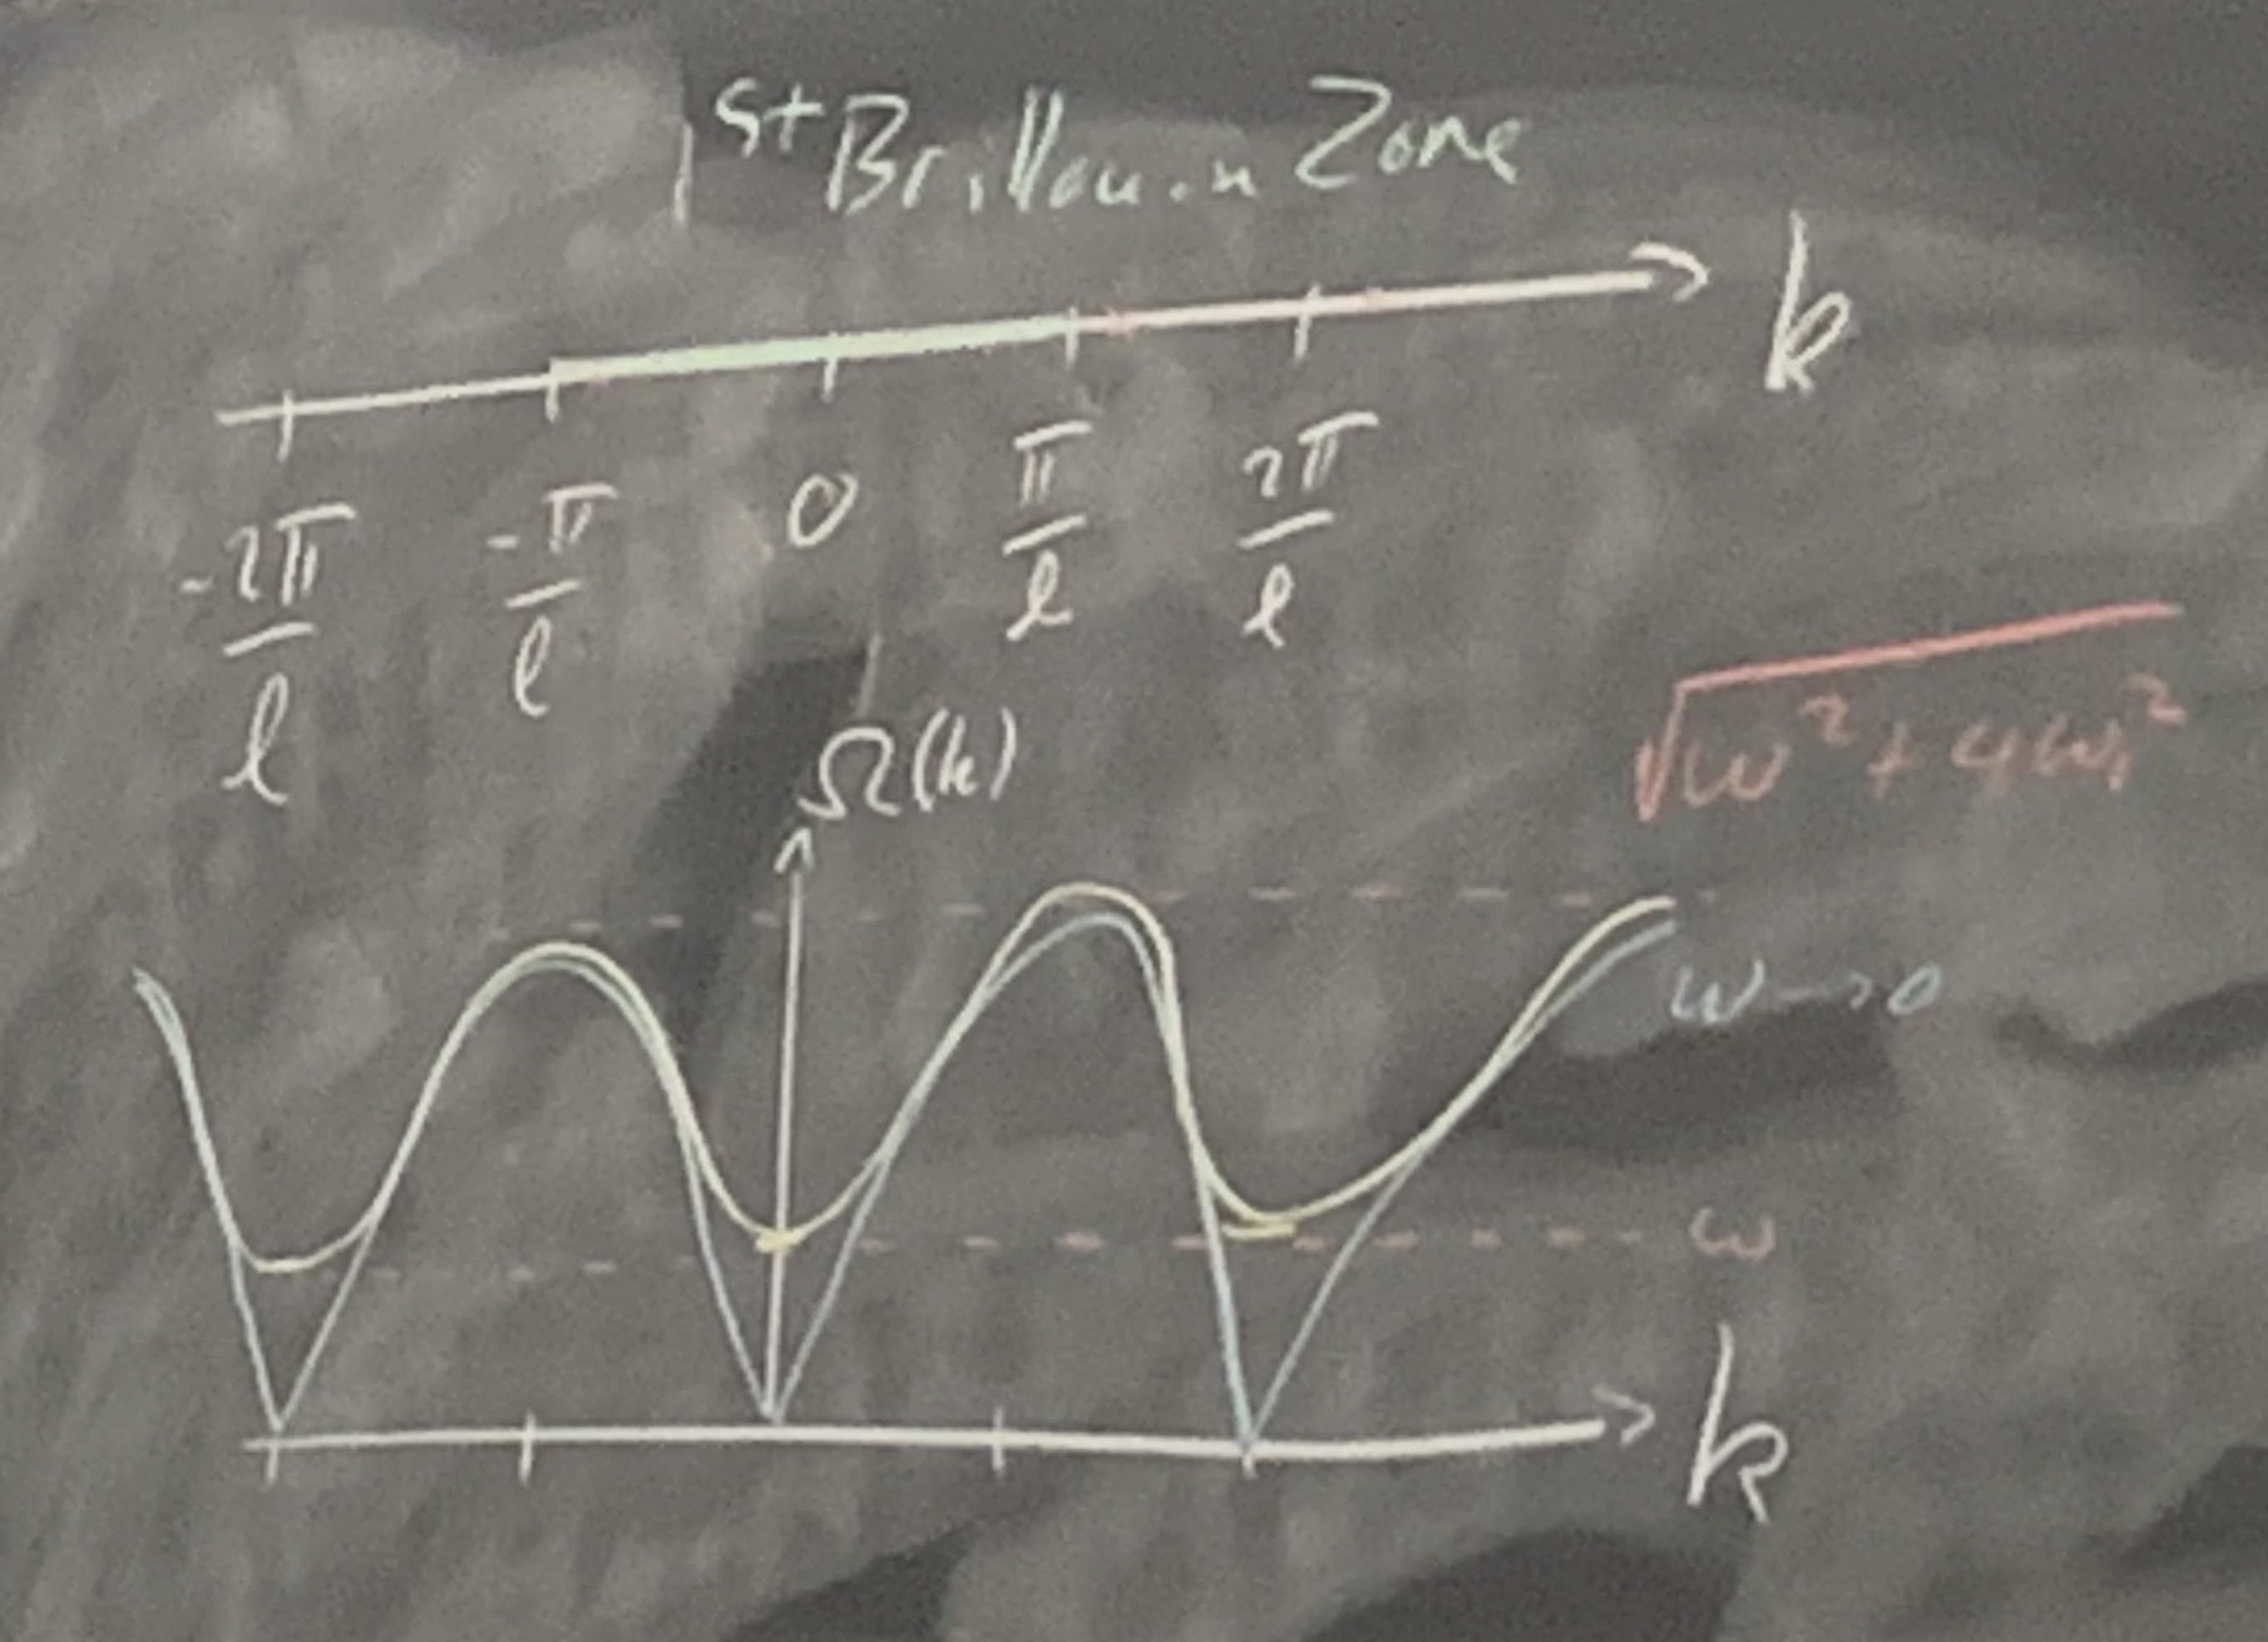
\includegraphics[width=\textwidth/2]{figures/lec_37_phonon_k.jpg}
    \caption{$ \Omega(k) $ in the first Brillouin zone.}
    \label{fig:omega_of_k_phonon}
\end{figure}



\end{document}
